%%%%%%%%%%%%%%%%%%%%%%% file template.tex %%%%%%%%%%%%%%%%%%%%%%%%%
%
% This is a general template file for the LaTeX package SVJour3
% for Springer journals.          Springer Heidelberg 2014/09/25
%
% Copy it to a new file with a new name and use it as the basis
% for your article. Delete % signs as needed.
%
% This template includes a few options for different layouts and
% content for various journals. Please consult a previous issue of
% your journal as needed.
%
%%%%%%%%%%%%%%%%%%%%%%%%%%%%%%%%%%%%%%%%%%%%%%%%%%%%%%%%%%%%%%%%%%%
%
% First comes an example EPS file -- just ignore it and
% proceed on the \documentclass line
% your LaTeX will extract the file if required
\begin{filecontents*}{example.eps}
%!PS-Adobe-3.0 EPSF-3.0
%%BoundingBox: 19 19 221 221
%%CreationDate: Mon Sep 29 1997
%%Creator: programmed by hand (JK)
%%EndComments
gsave
newpath
  20 20 moveto
  20 220 lineto
  220 220 lineto
  220 20 lineto
closepath
2 setlinewidth
gsave
  .4 setgray fill
grestore
stroke
grestore
\end{filecontents*}
%
\RequirePackage{fix-cm}
%
%\documentclass{svjour3}                     % onecolumn (standard format)
%\documentclass[smallcondensed]{svjour3}     % onecolumn (ditto)
%\documentclass[smallextended]{svjour3}       % onecolumn (second format)
%\documentclass[twocolumn]{svjour3}          % twocolumn
\documentclass[referee]{svjour3}

\smartqed  % flush right qed marks, e.g. at end of proof
%
%\usepackage{setspace}
%\onehalfspacing
\usepackage{amsmath}
\usepackage{graphicx}
\usepackage{lineno}
\usepackage{natbib}
\linenumbers
%
% \usepackage{mathptmx}      % use Times fonts if available on your TeX system
%
% insert here the call for the packages your document requires
%\usepackage{latexsym}
% etc.
%
% please place your own definitions here and don't use \def but
% \newcommand{}{}
%
% Insert the name of "your journal" with
% \journalname{myjournal}

%
\newcommand*\patchAmsMathEnvironmentForLineno[1]{%
\expandafter\let\csname old#1\expandafter\endcsname\csname #1\endcsname
\expandafter\let\csname oldend#1\expandafter\endcsname\csname end#1\endcsname
\renewenvironment{#1}%
{\linenomath\csname old#1\endcsname}%
{\csname oldend#1\endcsname\endlinenomath}}% 
\newcommand*\patchBothAmsMathEnvironmentsForLineno[1]{%
\patchAmsMathEnvironmentForLineno{#1}%
\patchAmsMathEnvironmentForLineno{#1*}}%
\usepackage{floatpag,mwe}
\usepackage[table]{xcolor}
\usepackage{subfig}
\usepackage{multicol}
\usepackage{afterpage}
\usepackage{color}
\definecolor{greytext}{gray}{0.5}
\definecolor{offyellow}{cmyk}{0, 0, 1, .2}
\usepackage{pifont}
\AtBeginDocument{%
\patchBothAmsMathEnvironmentsForLineno{equation}%
\patchBothAmsMathEnvironmentsForLineno{align}%
\patchBothAmsMathEnvironmentsForLineno{flalign}%
\patchBothAmsMathEnvironmentsForLineno{alignat}%
\patchBothAmsMathEnvironmentsForLineno{gather}%
\patchBothAmsMathEnvironmentsForLineno{multline}%
}

\begin{document}

\graphicspath{{./figures/}}


\title{The Effects of varying  two paramteters on idealized convective boundary layer entrainment%\thanks{Grants or other notes
%about the article that should go on the front page should be
%placed here. General acknowledgments should be placed at the end of the article.}
}

%\titlerunning{Short form of title}        % if too long for running head

\author{N.~A.~Chaparro \and P.~H.~Austin \and D.~G.~Steyn
         %etc.
}

%\authorrunning{Short form of author list} % if too long for running head

\institute{ P.~H.~Austin \at
              Department of Earth, Ocean, and Atmospheric Sciences, 
              The University of British Columbia, 
	      Room 2020, Earth Science Building,
              2207 Main Mall,
              Vancouver, BC, 
              V6T 1Z4 \\
              Tel.: +\\
              Fax: +\\
              \email{@eos.ubc.ca}           %  \\
%             \emph{Present address:} of F. Author  %  if needed
           %\and
           %S. Author \at
           %   second address
}

\date{Received: DD Month YEAR / Accepted: DD Month YEAR}
% The correct dates will be entered by the editor


\maketitle

\begin{abstract}
The fundamentals of convective boundary layer entrainment, such as the dependence of the entrainment rate and entrainment zone depth on the convective Richardson number, have been established but there is still unresolved discussion about the form of these relationships. Details regarding the structure of the entrainment zone continue to emerge. The variety of convective boundary layer height and entrainment zone depth definitions adds further complexity. The study described in here aims to join this ongoing discussion.\\

A dry, shear-free, idealized convective boundary layer in the absence of large scale winds was modeled using a large eddy simulation.  The use of a ten member ensemble enabled calculation of true ensemble averages and potential temperature fluctuations as well as providing smooth average profiles.  A range of convective Richardson numbers was achieved by varying the two principle external parameters: surface vertical heat flux and stable upper potential temperature lapse rate.  The gradient method for determining local convective boundary layer height based on the potential temperature profile, at a single horizontal point, was found to be unreliable so a multi-linear regression method was used instead.  Average height and entrainment zone depth were then defined based on the ensemble and horizontally averaged potential temperature profile.\\  

Distributions of the local heights determined using the multi-linear fit to the potential temperature profile were found to narrow with increased upper stability.  The relationships of average entrainment rate and entrainment zone depth to Richardson number showed behaviour in general agreement with theory and the results of other studies.  In particular, the results of a recent direct numerical simulation study were reproduced.  Furthermore both relationships showed a change in exponent which could be attributed to a change in entrainment mechanism as conective Richardson number increases.  The average potential temperature gradient in the upper convective boundary layer and entrainment zone was seen to depend on the upper potential temperature lapse rate, as was the positive downward moving temperature fluctuations at the convective boundary layer top.  Overall, the upper potential temperature lapse rate emerged as the dominant parameter influencing scaled entrainment zone depth, and potential temperature variance in the entrainment zone and upper convective boundary layer.   

\keywords{Convective boundary layer \and Entrainment \and Large eddy simulation \and Potential Temperature Profile}
\end{abstract}

\section{Introduction}
\label{intro}


\subsection{Convective boundary layer (CBL) entrainment}
\label{sec:cblent}
Boundary layer (BL) height and the prediction thereof are important for calculating the concentration of any atmospheric species within the ML as well as the sizes of the turbulent structures.  In combination with the level at which clouds condense (lifting condensation level) knowledge of entrainment zone (EZ) depth facilitates predictions pertaining to the formation of cumulus clouds \cite{WilStu}.  Parameterizations for both CBL growth and EZ depth are required in mesoscale and general circulation models (GCMs).  Furthermore it is an attractive goal to develop a robust set of scales for this region analogous to Monin-Obvukov Theory \citep{Stull-BLMetIntro, Traum11, SteynBaldHoff, StullNelEl, Sorbjan1}.\\

The daytime CBL over land starts to grow after sunrise when the surface becomes warmer than the air above it.  Coherent turbulent structures (thermals) begin to form and rise. The thermals rise to their neutral buoyancy level, overshoot, and then overturn or recoil.  Concurrently, warm stable air from the free atmosphere (FA) above is trapped or enveloped and subsequently mixed into the growing turbulent mixed layer (ML) \citep{Stull-BLMetIntro}.  This mixing at the top of the CBL is known as entrainment and the region over which it occurs, the EZ \citep{DearWill80}. A common, simplified conceptual model of this case is the dry, shear free CBL \citep{SullMoengStev, FedConzMir04, BrooksFowler2}. This model serves as an intellectually accessible way to understand the dynamic and complex CBL and its EZ.\\

The CBL grows by trapping pockets of warm stable air between
or adjacent to impinging thermal plumes.  \citep{Traum11} summarize two categories of CBL entrainment:\\

\begin{itemize}

\item{Non turbulent fluid can be engulfed between or in the overturning of thermal plumes. This kind of event has been supported by the visualizations in \cite{SullMoengStev}'s large eddy simulation (LES) study as well as in \cite{Traum11}'s observations. In both it appeared to occur under a weak inversion or upper lapse rate ($\gamma$)}

\item{
Impinging thermal plumes distort the inversion interface dragging wisps of warm stable air down at their edges or during recoil under a strong inversion or lapse rate. This type of event is supported by the findings  of both \cite{SullMoengStev} and \cite{Traum11}.}

\end{itemize}

Shear induced instabilities do occur at the top of the atmospheric boundary layer and in some laboratory studies of turbulent boundary layers, under conditions of very high stability, breaking of internal waves has been observed.  Entrainment via the former is relatively insignificant in strong convection, and the latter has not been directly observed in real or modeled atmospheric CBLs over the range of conditions considered here \citep{Traum11, SullMoengStev}.\\

The ML is fully turbulent but the top is characterized by stable air with intermittent turbulence due to the higher-reaching thermals. \cite{GarciaMellado} demonstrated that the EZ is subdivided in terms of length and buoyancy scales.  That is, the lower region is comprised of mostly turbulent air with pockets of stable warmer air that are quickly mixed, and so scales with the convective scales. Whereas the upper region is mostly stable apart from the impinging thermals so scaling here is more influenced by the lapse rate ($\gamma$).  In the EZ the vertical heat flux, $\overline{w^{'}\theta^{'}}$, has opposite sign relative to that in the ML.  The fast updraughts are now relatively cool $\overline{w^{'+}\theta^{'-}}$.  In their analysis of the four $\overline{w^{'}\theta^{'}}$ quadrants \cite{SullMoengStev} concluded that the net dynamic in this region is downward motion of warm air ($\overline{w^{'-}\theta^{'+}}$) from the FA since the other three quadrants effectively cancel.\\

\subsection{Modeling CBL entrainment}

\subsubsection{Bulk models}
\label{subsubsec:bulkmod}

Bulk  models for the CBL based on average, vertical profiles of ML quantities can be subdivided into: (i) zero-order jump and (ii) first-(and higher) order jump bulk models.  Increased order corresponds to increasing complexity in the shape of the  $\overline{\theta}$ and $\overline{w^{'}\theta^{'}}$ profiles at the top of the ML.\\
 
Zero-order jump bulk models assume a ML of uniform potential temperature ($\overline{\theta}_{ML}$) topped by an infinitesimally thin layer across which there is a temperature jump ($\delta \theta$) and above which is a constant lapse rate.  The assumed vertical heat flux, $\overline{w^{'}\theta^{'}}$, decreases linearly from the surface up, reaching a maximum negative value $(\overline{w^{'}\theta^{'}})_{h}$ .  This is a constant proportion of the surface value, usually $-0.2(\overline{w^{'}\theta^{'}})_{s}$ (see Section 4 in \cite{Tennekes73} for a discussion). At the temperature inversion, $\overline{w^{'}\theta^{'}}$ jumps to zero across the infinitesimally thin layer.  Equations for the evolution of CBL height, $\overline{\theta}_{ML}$ and $\delta \theta$ are derived on this basis \citep{Tennekes73}.\\

First (and higher) order jump models assume an EZ of finite depth at the top of the ML, defined by two heights:  the top of the ML ($h_{0}$) and the point where FA characteristics are resumed ($h_{1}$).  The potential temperature jump ($\Delta \theta$) is then the difference accross the EZ.  Derivations are more complex and involve assumptions about the EZ \citep{Betts74, BatchGryn, Stull73, Deardorff79, FedConzMir04}.\\

\subsubsection{Numerical simulations}
\label{subsec:numsim}

Numerical simulation of the CBL is carried out by solving the Navier Stokes equations, simplified according to a suitable approximation, on a discrete grid.  Types of simulations can be grouped according to the scales of motion they resolve.  In direct numerical simulations (DNS) such as that used by \cite{GarciaMellado} the full range of spatial and temporal turbulence are resolved from the size of the domain down to the smallest dissipative scales i.e. the Kolmogorov micro-scales \citep{Kolmog}.  This requires a dense numerical grid and so can be computationally prohibitive.\\

In an LES motion on scales smaller than twice or more of the grid spacing is filtered out and parameterized by a sub-grid scale closure model. LES has increasingly been used to better understand the CBL since \cite{Deardorff72} devised it for this purpose.  \cite{SullMoengStev}, \cite{FedConzMir04}, \cite{EbSchu} and \cite{BrooksFowler2} used it to study the structure and scaling behaviour of the EZ.\\

\subsection{CBL entrainment scales and scaling relations (parametrizations)}
\label{subsec:scales}
\subsubsection{Length scale ($h$)}
\label{subsubsec:}

\cite{Deardorff72} demonstrated that dominant turbulent structures in penetrative convection scale with CBL height, which he referred to as the inversion height but measured as the height of minimum vertical heat flux.  Since then, the distinction between the two has been clarified \citep{SullMoengStev} and here $h$ refers strictly to the height of maximum average potential temperature gradient. There are alternatives. For example turbulence based definitions, such as the velocity variance and the distance over which velocity is correlated with itself, represent the current turbulent dynamics rather than the recent turbulence history as does $h$ \citep{Traum11}.\\

\subsubsection{Deardorff (convective) velocity scale ($w_{*}$)}
\label{subsubsec:convel}

\cite{Deardorff70} confirmed that the convective velocity scale

\begin{equation}
w_{*} = \left( \frac{gh}{\overline{\theta}}(\overline{w^{'}\theta^{'}})_{s} \right)^{\frac{1}{3}},
\end{equation}


 effectively scaled the local vertical turbulent velocity fluctuations ($w^{'}$) in the CBL.  \cite{Sorbjan1} supports this, even at the CBL top.  The CBL entrainment rate ($w_{e} = \frac{dh}{dt}$, neglecting large scale subsidence) depends on the magnitude of $w^{'}$ which is driven by $(\overline{w^{'}\theta^{'}})_{s}$. Stability aloft suppresses $\frac{dh}{dt}$ so the influence of $\gamma$ is indirectly accounted for via $h$ in $w_{*}$.\\

\subsubsection{Temperature scales ($\theta_{*}$ and $\delta h \gamma$)}
\label{subsubsec:tempscales}

CBL temperature fluctuations $\theta^{'}$ are influenced by $\overline{w^{'}\theta^{'}}$ from both the surface and the CBL top.
\cite{Deardorff70} showed that an effective scale based on the convective velocity scale is

\begin{equation}
\theta_{*} = \frac{(\overline{w^{'}\theta^{'}})_{s}}{w_{*}},
\end{equation} 

whereas \cite{Sorbjan1} showed that with proximity to the CBL top the effects of FA stability $\gamma$ become more important.  An alternative potential temperature scale for the EZ ($\delta h \gamma$) is demonstrated in Fig. \ref{fig:deltahgamma}. This is the difference in the initial or background potential temperature ($\overline{\theta}_{0}$) across the upper part of the EZ, i.e. between $h$ and $h_{1}$.      

\begin{figure}[htbp]
    \centering
    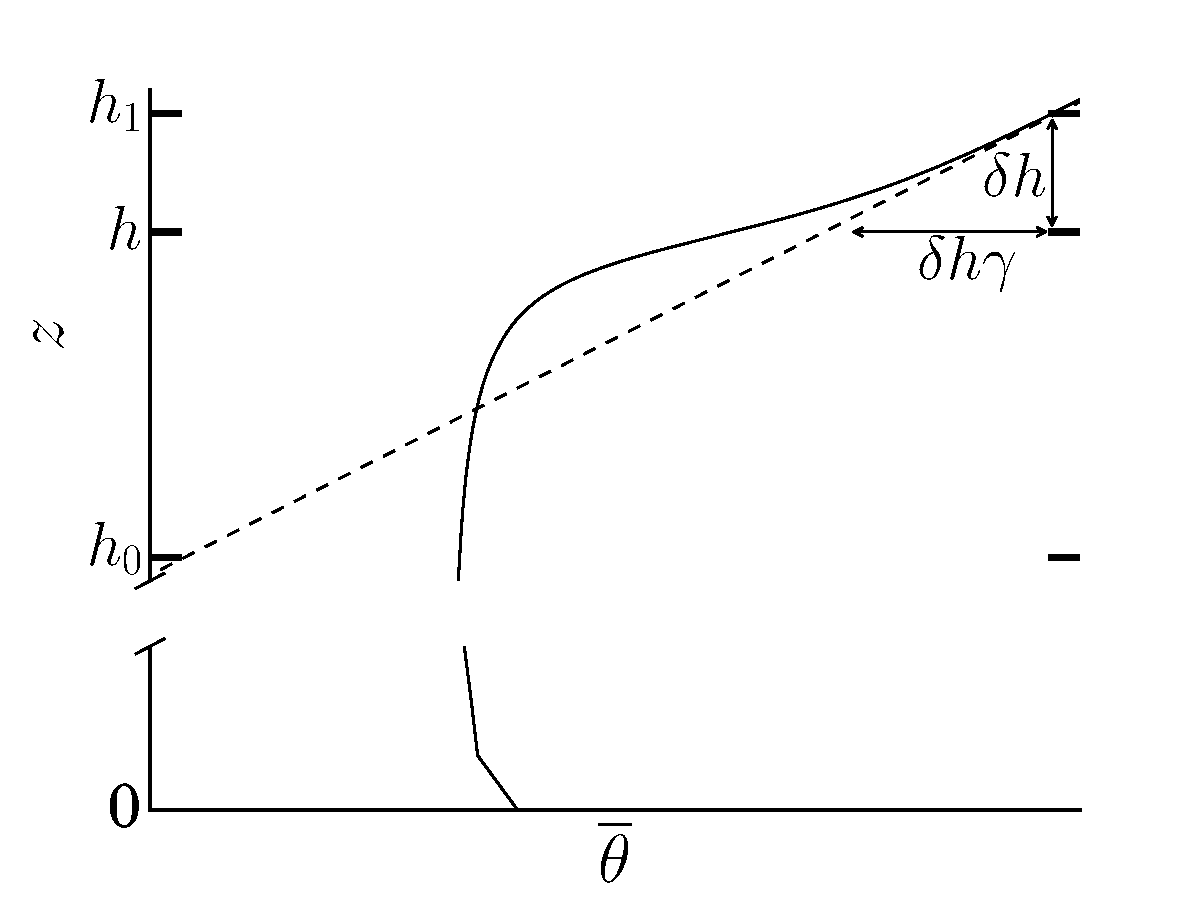
\includegraphics[scale=.32]{figures/deltah_gamma.pdf}
    \caption[Alternative Potential Temperature Scale for the EZ]{Representation of the difference in $\overline{\theta}_{0}$ across the upper part of the EZ, $\delta h \gamma$ where $\delta h = h_{1} - h$. This serves as an alternative to the convective potential temperature scale $\theta_{*}$. $h_{1}$, $h$ and $h_{0}$ are the upper EZ limit, CBL height and the lower EZ limit respectively. The solid line is the average potential temperature profile and the dashed line is the initial or background potential temperature profile.}
    \label{fig:deltahgamma}   % label should change
\end{figure}

\subsubsection{Convective richardson number ($Ri$)}
\label{subsubsec:}


The convective Richardson number is a simplifed, bulk approximation to the flux Richardson number \citep{Stull-BLMetIntro}.  The natural choice of length and velocity and temperature difference scales are $h$, $w_{*}$ and $\Delta \theta$:

\begin{equation}
Ri = \frac{\frac{g}{\overline{\theta}} \Delta \theta h}{w^{*2}}.
\end{equation}

$\Delta \theta$ can be replaced by $\delta \theta$ as in \cite{FedConzMir04} and \cite{GarciaMellado}.  $Ri$ can also be obtained by considering the principal forcings of the system, or from non-dimensionalizing the entrainment relation derived analytically \citep{Tennekes73, Deardorff72}. It is central to any study on CBL entrainment \citep{SullMoengStev, FedConzMir04, Traum11, BrooksFowler2}.

\subsubsection{Relationship of entrainment zone depth to $Ri$}

A relationship of the scaled entrainment zone EZ depth to $Ri$

\begin{equation}\label{eq:dhvsri}
\frac{\Delta h}{h} \propto Ri ^{b}
\end{equation}

where $b=1$ is arrived at by considering the deceleration of a thermal
as it overshoots its neutral buoyancy level \cite{StullNelEl}.  Alternatively, \cite{Boers89} integrated the internal, potential and kinetic energy over a hydrostatic atmosphere to obtain a value of $b=\frac{1}{2}$.

\subsubsection{Relationship of entrainment rate to $Ri$}
\label{subsec:erri}
The relationship between scaled entrainment rate and the buoyancy Richardson number ($Ri$)

\begin{equation}\label{eq:ervsri}
\frac{w_{e}}{w_{*}} \propto Ri^{a}
\end{equation}

is derived according to the zero-order jump bulk model through thermodynamic arguments, or by integration of the conservation of enthalpy or turbulent kinetic energy equations over the growing CBL \citep{Tennekes73, Deardorff79, FedConzMir04}. It has been verified in numerous laboratory and numerical studies \citep{DearWill80, SullMoengStev, FedConzMir04, BrooksFowler2}, but there is still some unresolved discussion as the the exact value of a.  Two possible values are $-\frac{3}{2}$ and $-1$ \citep{Traum11}.  \cite{Turner86} suggested that the former occurs at high stability when buoyant recoil of impinging thermals becomes more important than their convective overturning.  Adding further complexity to this discussion, \cite{FedConzMir04} arrived a similar power law relationship ($a = -1.7$) through defining the $\theta$ jump across the EZ rather than at $h$.\\

\section{Tools and approach}

\subsection{LES set up}

The LES used in this study, System for Atmospheric Modelling (SAM), is described in \cite{KhairRand}.

\subsubsection{Domain and grid sizes}
The dry shear free CBL and EZ was modelled using SAM.  An ensemble of 10 cases was run to obtain true ensemble averages and turbulent potential temperature fluctuations ($\theta^{'}$). Each case had a domain of area 3.2 x 4.8 Km$^{2}$.  Grid numbers $n_{x}$, $n_{y}$ were chosen based on the optimal distribution across processor nodes. The vertical grid ($n_{z}=312$) was of higher resolution around the entrainment zone ($\Delta z = 5$m), lower below ($\Delta z = 25$m) and stretched above it ($\Delta z = 10 \ to \ 100 $m). This was guided by \cite{SullPat}'s LES resolution study of the CBL that showed how grid size effects, the shapes of the average profiles in particular around the EZ, as well as the extent of the inertial turbulence scale sub-range.\\

\subsubsection{Initial conditions}

The runs were initialized with a constant $(\overline{w^{'}\theta^{'}})_{s}$ acting against a uniform $\gamma$.  Thus, the  $\theta$ jump arose from the overshoot of the thermals, rather than being initially imposed as in \cite{SullMoengStev} and \cite{BrooksFowler2}.  The 7 runs differ from each other based on surface heat flux ( $(\overline{w^{'}\theta^{'}})_{s}$ ) and initial potential temperature lapse rate ($\gamma$) and are summarized accordingly in Table \ref{fig:tableofruns}.

\begin{table}[!ht]
\caption{Runs in terms of $\overline{w^{'} \theta^{'}_{s}}$ and initial Lapse Rate $\gamma$.  Runs at weaker $\gamma$ and higher $\overline{w^{'} \theta^{'}_{s}}$ would have required a larger region of high vertical resolution, so were avoided.  The coloured symbols will be used in plots throughout.}
    \begin{center}
    \begin{tabular}{ | l | l | l | l |}
    \hline
    $\overline{w^{'}\theta^{'}_{s}}$ / $\gamma$ & 10 (Kkm$^{-1}$) & 5 (Kkm$^{-1}$) & 2.5 (Kkm$^{-1}$) \\ \hline
     150 (Wm$^{-2}$)& \hspace{2mm} {\color{red} \ding{116}} 150/10 &\hspace{3   mm}{\color{red} \ding{108}} 150/5\footnotemark &  \\ \hline
     100 (Wm$^{-2}$)& \hspace{2mm} {\color{black} \ding{116}} 100/10 & \hspace{2mm} {\color{black} \ding{108}} 100/5 & \\ \hline
     60 (Wm$^{-2}$) & \hspace{2mm} {\color{offyellow} \ding{116}} 60/10 & \hspace{2mm} {\color{offyellow} \ding{108}} 60/5 & \hspace{2mm} {\color{offyellow} \ding{72}} 60/2.5\\ \hline
\end{tabular}
\label{fig:tableofruns}   
\end{center}    
\end{table}
\footnotetext{Incomplete run: EZ exceeded high resolution vertical grid after 7 hours}

\subsection{Comparison of domain, grid size and initial conditions}

\cite{SullPat} found that the shapes of the average potential temperature ($\overline{\theta}$) and heat flux ($\overline{w^{'}\theta^{'}}$) profiles, as well as the measured CBL height vary depending on grid size.  The resolution at which convergence began is listed in Table \ref{table:gridcomp}.  Lower resolution resulted in a higher CBL and relatively larger EZ based on the $\overline{\theta}$ and $\overline{w^{'}\theta^{'}}$ profiles.  Overall they concluded that vertical resolution was critical.  This compliments the conclusion \cite{BrooksFowler2} reached when discussing their resolution test.  That is, to capture the steep vertical gradients in the EZ requires high vertical resolution. \\

Here, fast fourrier transform (FFT) energy spectra of the turbulent velocities at the top of the ML show a substantial resolved inertial subrange giving confidence in the choice of horizontal grid size used. In the EZ where turbulence is intermittent, the dominant energy containing structures are smaller, and decay to the smallest resolved turbulent structures is steeper. Two dimensional horizontal slices of potential temperature and turbulent vertical velocity perturbations at $h_{0}$, $h$ and $h_{1}$ show several coherent impinging thermals at any given time after 2 hours, indicating that realistic turbulence was being simulated.\\

\begin{table}[htbp]
\caption[Comparison of Grid-Sizes used in similar Studies]{Grid spacing around the EZ used in comparable LES studies. Those used for resolution tests are not listed here.  For \cite{SullPat}'s resolution study the grid sizes, at which profiles within the EZ and CBL height evolution began to converge, are listed.}

    \begin{tabular}{p{4cm} p{2cm} p{2cm}}
Publication & $\Delta x$, $\Delta y$, $\Delta z$ & Horizontal \\
 & in the EZ (m) & Domain (km$^{2}$) \\ \hline
      \cite{SullMoengStev}& 33, 33, 10 & 5 x 5 \\ 
      \cite{FedConzMir04}& 100, 100, 20 & 5 x 5 \\ 
      \cite{BrooksFowler2}& 50, 50, 12 & 5 x 5 \\
      \cite{SullPat} &  20, 20, 8 & 5 x 5\\
      This study & 25, 25, 5 &  3.4 x 4.8\\ \hline       
    \end{tabular}
%}
\label{table:gridcomp}   
%\end{center}    
\end{table}

The principal parameter describing the balance of forces in dry, idealized CBL entrainment is the Richardson number ($Ri$) and its magnitude depends on the way in which the $\theta$ jump is defined.  Varying the $\theta$ jump definition causes identical conditions to be described by different $Ri$ values.  In this study the dependence of $Ri$ on variation in $\gamma$ was evident.  \cite{BrooksFowler2} and \cite{SullMoengStev} imposed a $\theta$ jump of varying strength topped by a constant $\gamma$.  Whereas \cite{FedConzMir04} initialized with a layer of uniform $\theta$.  They varied $\gamma$ and kept $\overline{w^{'}\theta^{'}}_{s}$ constant for each run.  Their initial conditions, definitions of the $\theta$ jump and $Ri$ range are directly comparable to those of this study.  \cite{BrooksFowler2} and \cite{SullMoengStev} defined CBL height, the EZ and $\theta$ jump as averages of local values determined based on tracer profiles.  So the resulting $Ri$ values are quite different.    

\begin{table}[htbp]
\caption[Initial Conditions used in comparable LES Studies]{Initial Conditions used in comparable LES Studies}

  
    \begin{tabular}{ p{4cm} p{1.4cm} p{1.4cm} p{1.7cm} p{1.8cm}}
    
Publication & $\overline{w^{'}\theta^{'}}_{s}$& $\gamma$& Initial $\theta$ & $Ri$ \\ 
& $Wm^{-2}$ & $Kkm^{-1}$ & Jump K & range \\ \hline
      \citeauthor{SullMoengStev} (\citeyear{SullMoengStev}) & 20 - 450& 3  &.436 - 5.17 & 1 - 100\\
      \citeauthor{FedConzMir04} (\citeyear{FedConzMir04}) & 300 & 1 - 10 & NA & 10 - 40\\ 
      \citeauthor{BrooksFowler2} (\citeyear{BrooksFowler2}) &  10 -100 &  3& 1 - 10 &10 - 100 \\
      This study & 60 - 150 & 2.5 - 10& NA & 10 - 30\\ \hline 
      
    \end{tabular}
%}
\label{table:initconditcomp}   

\end{table}

\subsection{Tri-linear fit for local CBL height}
In their LES study \cite{BrooksFowler2} encountered inconsistencies when determining the EZ boundaries from the average tracer profile.  Although their tracer profile was quite different to a simulated CBL $\overline{\theta}$ profile, this could serve as cautionary note.  \cite{SullMoengStev} determined local CBL height, i.e. that at an indivitual horizontal point, by locating the point of maximum $\frac{\partial \theta}{\partial z}$.  Analysis of the resulting distributions showed dependence of standard deviation and skewness on $Ri$.  The normalized standard deviation decreased with increased $Ri$ whereas skewness was almost bimodal; being negative at high $Ri$ and positive and low $Ri$.  Initially in this study, a similar method was applied and local CBL height distributions with lower $Ri$ were found to have positive skew.  Upon exhaustive inspection of local vertical $\theta$  profiles such as those in Fig. \ref{fig:rssfitshigh}, it became evident that at certain horizontal points high gradients well into the free atmosphere exceeded those within the EZ.  Locating the local ML height ($h^{l}_{0}$) using a multi-linear regression method based on that of \citep{Vieth} and described in \citep{NChap14} proved more reliable than the gradient method discussed above.  As shown in Fig. \ref{fig:rssfitshigh} a line is fit to each of the ML, EZ an FA.\\
  
\begin{figure}[htbp]
\begin{minipage}[b]{0.5\linewidth}
        %
        \subfloat[]{\label{main:a}
                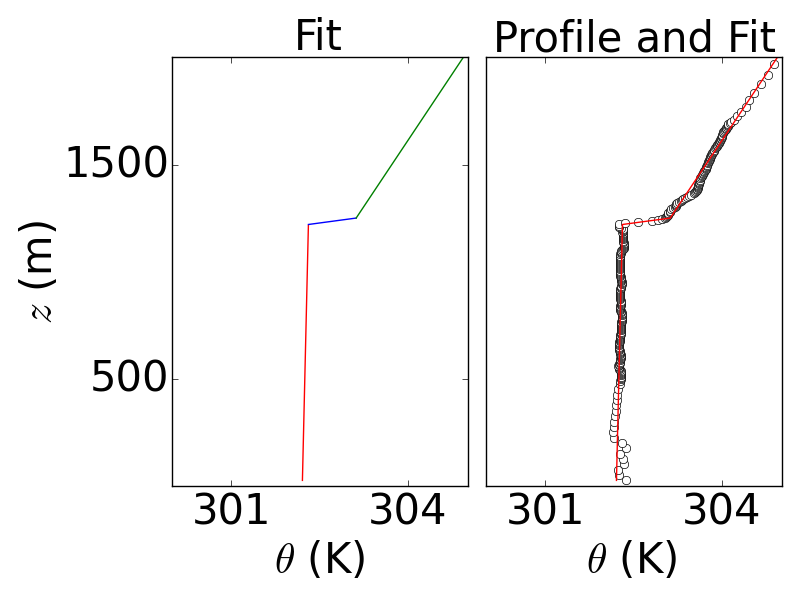
\includegraphics[scale=.31]{figures/rss_fit_high}}\\
        \end{minipage}             
\quad
\begin{minipage}[b]{0.5\linewidth}
        \subfloat[]{\label{main:b}          
          
                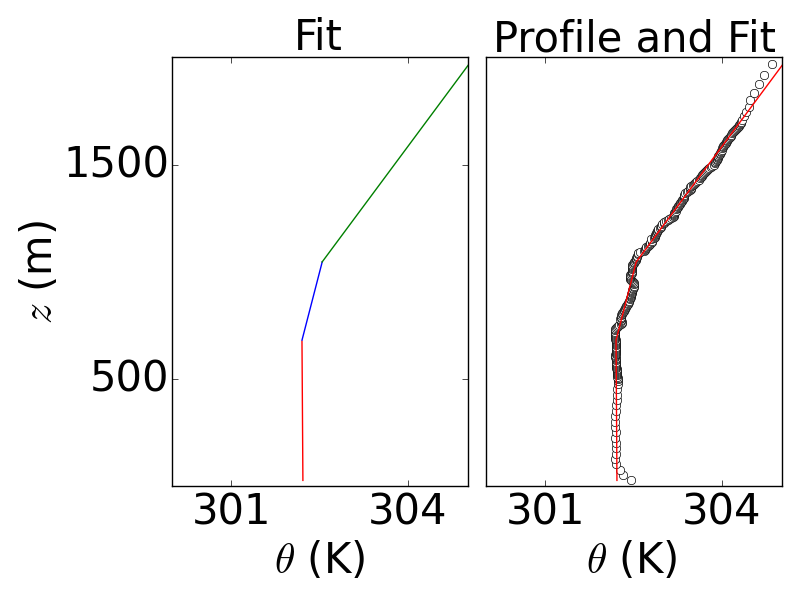
\includegraphics[scale=.31]{figures/rss_fit_low}}
       
       \end{minipage}
\caption[High local ML ]{Local vertical $\theta$ profiles with 3-line fit for the 60/2.5 run at a point where $h^{l}_{0}$ (a) is high and (b) low.}
\label{fig:rssfitshigh}
\end{figure}

%\begin{figure}[htbp]
%\begin{minipage}[b]{0.5\linewidth}
 %       \subfloat[]{\label{main:a}
   %             \includegraphics[scale=.31]{}}
  %      \end{minipage}             
%\quad
%\begin{minipage}[b]{0.5\linewidth}
%\vspace{-20mm}
 %       \subfloat[]{\label{main:b}              
  %        \includegraphics[scale=.31]{}}
   %    \end{minipage}
%\caption[]{}
        
        %\label{fig:rssfitshigh}
%\end{figure}

\subsection{Definitions based on scaled ensemble and horizontally averaged profiles}

Here the CBL height ($h$) is defined as the location of maximum scaled vertical $\overline{\theta}$ gradient as in Figure \ref{fig:hdefs}.  The lower and upper EZ boundaries ($h_{0}$ and $h_{1}$) are then the points at which $\frac{\frac{\partial \overline{\theta}}{\partial z}}{\gamma}$ significantly exceeds zero and where it resumes $1$.  The lower boundary requires a choice of a threshold value which should be small, positive and less than $1$. \cite{FedConzMir04} and \cite{BrooksFowler2} defined the EZ in terms of the vertical $\overline{w^{'}\theta^{'}}$ profiles as in Figure \ref{fig:hdefs} but disagreed on the shape of the relationship of scaled EZ depth to $Ri$ (equation 2.1).  As well as observing this relationship using the height definitions based on the $\frac{\frac{\partial \overline{\theta}}{\partial z}}{\gamma}$ profile, definitions based on the $\frac{\overline{w^{'}\theta^{'}}}{(\overline{w^{'}\theta^{'}})_{s}}$ profile are applied for comparison with \cite{BrooksFowler2}, \cite{FedConzMir04} and \cite{GarciaMellado}.\\  

\begin{figure}[htbp]
\thisfloatpagestyle{empty}
\begin
{minipage}[b]{0.5\linewidth}
         \subfloat[]{\label{main:a}
                \includegraphics[scale=.22]{ML_Height_hist_5}
}\\
\end{minipage}
\quad
\begin{minipage}[b]{0.5\linewidth}
         \subfloat[]{\label{main:b}
                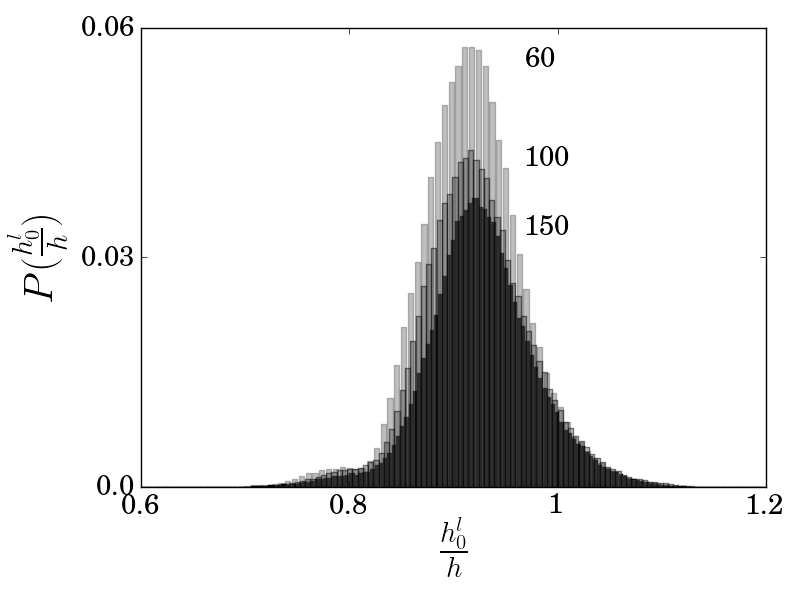
\includegraphics[scale=.22]{Scaled_ML_Height_hist_5}
}\\     
        
\end{minipage}
\caption[Local ML Height Distributions]{Histograms of local ML heights ($h^{l}_{0}$) for the three runs with $\gamma = 5$ Kkm$^{-1}$ are shown in (a). Darker shading corresponds to increase in $(\overline{w^{'}\theta^{'}})_{s}$, i.e. $60 - 150$ Wm$^{-1}$ per plot annotation. Counts are per height bin and bin-widths are 5m.  Probability distributions of scaled local ML height ($\frac{h^{l}_{0}}{h}$) for the three runs with $\gamma = 5$Kkm$^{-1}$ are shown in (b). The probabilities are the proportions in each scaled height bin. Both sets of plots are taken at 5 hours.}    
\label{fig:localh}
\end{figure}

\begin{figure}[htbp]
    \centering
    
    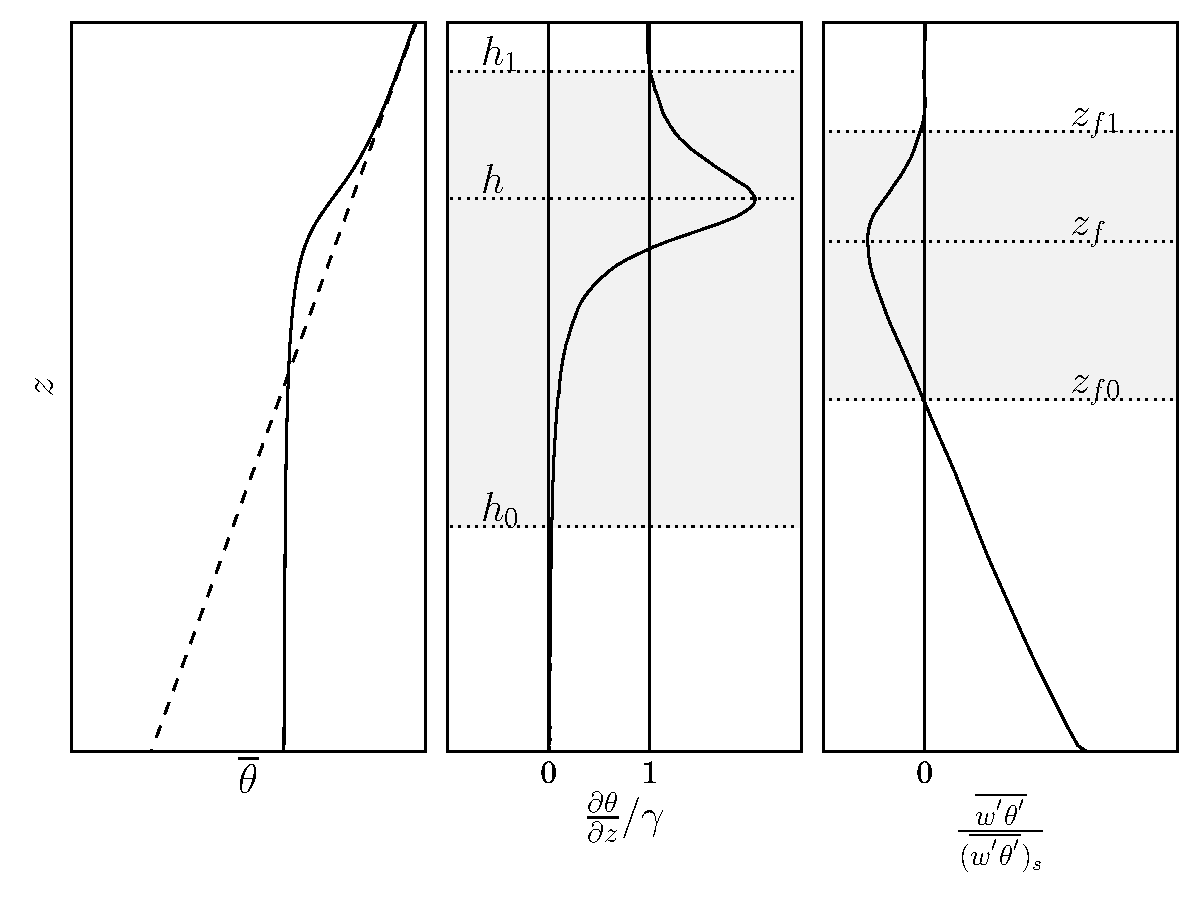
\includegraphics[scale=.5]{figures/height_defs.pdf}
    \caption[Height Definitions]{Height definitions based on the scaled average vertical profiles. The dashed line in the far left pannel represents the initial $\overline{\theta}$ profile. $z_{f0}$, $z_{f}$ and $z_{f1}$ are the points at which the $\frac{\overline{w^{'}\theta^{'}}}{(\overline{w^{'}\theta^{'}})_{s}}$ profile first crosses zero, is minumum and resumes zero at the top of the EZ.}
    \label{fig:hdefs} 
\end{figure}

\begin{table}[htbp]
\caption[Height definitions]{Definitions based on the vertical $\overline{\theta}$ profile in Figure \ref{fig:hdefs}. To obtain those based on the $\overline{w^{'}\theta^{'}}$ profile, replace $h_{0}$, $h$ and $h_{0}$ with $z_{f0}$, $z_{f}$ and $z_{f1}$}


    \begin{tabular}{p{1.cm} p{3.cm} p{3cm} p{2.5cm}}
    
      CBL Height & ML $\overline{\theta}$ & $\theta$ Jump &$     Ri $\\ \hline 
       $h$ & $\overline{\theta}_{ML} = \frac{1}{h}\int^{h}_{0}\overline{\theta}(z)dz$ & $\Delta \theta=\overline{\theta}(h_{1})-\overline{\theta}(h_{0})$ &      Ri $_{\Delta}=\frac{\frac{g}{\overline{\theta}_{ML}}\Delta \theta h}{w^{*2}}$  \\ [.3cm] 
        
       & &$\delta \theta = \overline{\theta}_{0}(h)- \overline{\theta}_{ML}$ & \    Ri $_{\delta}=\frac{\frac{g}{\overline{\theta}_{ML}} \delta \theta h}{w^{*2}}$ \\ \hline
      \end{tabular}

\label{tab:reldefs}   
    
\end{table}

\section{Results}
\subsection{EZ structure}

\subsubsection{Local CBL heights ($h_{0}^{l}$)}
\label{subsubsec:loccblh}

The distribution of $h_{0}^{l}$ represents the range over which CBL height varies in space so relates to the depth of the entrainment zone (EZ).  In Fig. \ref{fig:localh} (a) it widens with increasing $(\overline{w^{'}\theta^{'}})_{s}$ and is seen to narrow with increasing $\gamma$ in analysis not shown here.  When scaled by $h$, the local ML height distribution narrows with increased $\gamma$.  The upper boundary seems to be constant at about 1.1($\times h$) , whereas the lower boundary increases.  When $h_{0}^{l}$s are lower and their distribution is narrower, the scaled versions have relatively larger spacing between bins and so higher numbers in each bin. In Figure \ref{fig:localh} (b), at higher $(\overline{w^{'}\theta^{'}})_{s}$ there are fewer $\frac{h_{0}^{l}}{h}$ values with higher probabilities, but the width of the distributions is more or less constant regardless of $(w^{'}\theta^{'})_{s}$.\\


\begin{figure}[htbp]
\thisfloatpagestyle{empty}
\begin
{minipage}[b]{0.5\linewidth}
         \subfloat[]{\label{main:a}
                \includegraphics[scale=.22]{figures/ML_Height_hist_5}
}\\
\end{minipage}
\quad
\begin{minipage}[b]{0.5\linewidth}
         \subfloat[]{\label{main:b}
                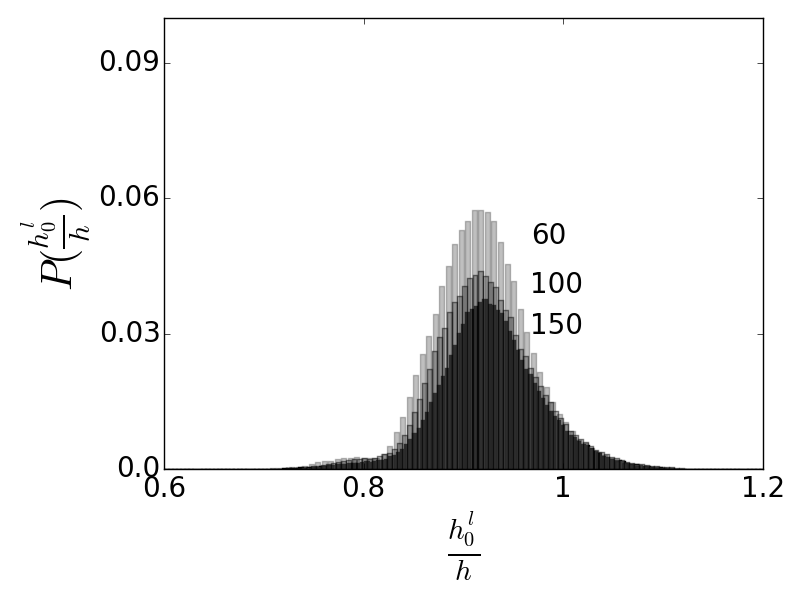
\includegraphics[scale=.22]{figures/Scaled_ML_Height_hist_5}
}\\     
        
\end{minipage}
\caption[Local ML Height Distributions]{Histograms of local ML heights ($h^{l}_{0}$) for the three runs with $\gamma = 5$ Kkm$^{-1}$ are shown in (a). Darker shading corresponds to increase in $(\overline{w^{'}\theta^{'}})_{s}$, i.e. $60 - 150$ Wm$^{-1}$ per plot annotation. Counts are per height bin and bin-widths are 5m.  Probability distributions of scaled local ML height ($\frac{h^{l}_{0}}{h}$) for the three runs with $\gamma = 5$Kkm$^{-1}$ are shown in (b). The probabilities are the proportions in each scaled height bin. Both sets of plots are taken at 5 hours.}
    
\label{fig:localh}

\end{figure}

The lowest $\frac{h^{l}_{0}}{h}$ decrease with decreased stability ($Ri$) causing increased negative skew. This, combined with a widening of the distribution agrees, with the findings of \cite{SullMoengStev} and supports the results based on the average profiles to be discussed later.  The approximate scaled EZ based on the $\frac{h^{l}_{0}}{h}$ distributions is about 0.2 - 0.4 whereas that based on distributions of local maximum tracer gradients by  \cite{BrooksFowler2} was smaller (0.05 - 0.2).  However, the local maximum gradient of the tracer profile would likely be within the EZ at points outside an actively impinging plume and so higher than $h^{l}_{0}$ defined here and the distributions could be quite different. \\  

\subsubsection{Local $w$ and $\theta$ fluctuations}
\label{subsubsec:locfluc}

\cite{SullMoengStev} decomposed $w^{'}\theta^{'}$ into four quadrants and used this combined with local flow visualizations to show how CBL thermals impinge and draw down warm air from above. \cite{MahrtPaum} used 2 dimensional contour plots of local $w^{'}$ and $\theta^{'}$ measurements to analyze their joint distributions.  \cite{Sorbjan1} concluded that in the EZ, $\theta^{'}$ is strongly influenced by $\gamma$  whereas $w^{'}$ is practically independent thereof.  Influenced by these three studies, 2 dimensional histograms at $h$ and so within the EZ, are used here to see how distributions of local $w^{'}$ and $\theta^{'}$ are effected by changes in $\gamma$ and $(\overline{w^{'}\theta^{'}})_{s}$ .  The effects of $\gamma$ are magnified by applying the convective scales, $\theta_{*}$ and $w_{*}$ and the entrained air at $h$ is focused on specifically by looking at the downward moving warm potential temperature fluctuations.\\    

The two-dimensional histograms of $\theta^{'}$ and $w^{'}$, at each horizontal point in each ensemble case, for all runs at $h$ are plotted as in Fig. \ref{fig:margdist}.  Bootstrapped standard deviations are presented in Tables \ref{tab:stdevw} and \ref{tab:stdevtheta} to show the influence of changes in $(\overline{w^{'} \theta^{'}})_{s}$ and $\gamma$.  The scaled two-dimensional histograms of $w^{'}$ and $\theta^{'}$ for each run are plotted in Figure \ref{fig:scaled_fluxquadhs}.\\

\begin{figure}[htbp]
\centering
 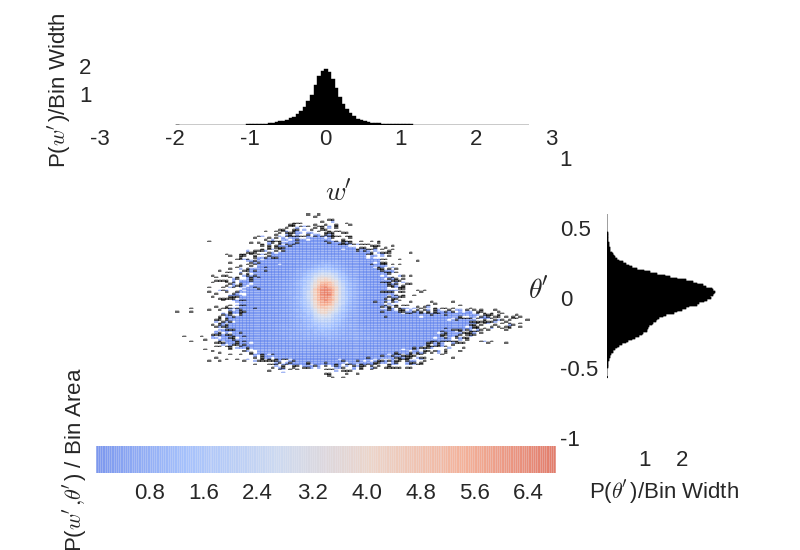
\includegraphics[scale=.5]{figures/marg_dist}                 
\caption[]{Two dimensional histogram of $w^{'}$ and $\theta^{'}$ at $h$ with marginal distributions. There are 100 bins for each and bin-widths are 0.047ms$^{-1}$ and 0.0117K for $w^{'}$ and $\theta^{'}$ respectively.}
\label{fig:margdist}
\end{figure}

Distributions of both $w^{'}$ and $\theta^{'}$ widen with increasing $(\overline{w^{'}\theta^{'}})_{s}$.  Whereas that of $\theta^{'}$ increases only slightly with increasing stability ($\gamma$).  As expected, increased $\gamma$ inhibits both upward and downward $w^{'}$. The scaled distributions in Figure \ref{fig:scaled_fluxquadhs} show damping of $w^{'}$ where potential temperature fluctuations are positive. Concurrently, the coolest negative $\frac{\theta^{'}}{\theta_{*}}$ become less cool, and the warmest become warmer.  So the $\frac{\theta^{'}}{\theta_{*}}$ distribution shifts positively with increasing $\gamma$.\\ 


\begin{table}[htbp]
\caption[]{Bootstrapped average Standard Deviations with 90$\%$ confidence intervals by run for the distributions of $w^{'}$ at $h$}
 

    \begin{tabular}{ p{2.1cm} p{2.2cm}  p{2.2cm}  p{2.2cm} p{2.2cm} }
    
     $\overline{w^{'}\theta^{'}}_{s}$ / $\gamma$ & 10Kkm$^{-1}$ & 5Kkm$^{-1}$  & 2.5Kkm$^{-1}$   \\ \hline
     150 (Wm$^{-2}$)& 0.363 [.361, .365]& 0.427 [.425, .430] &  \\
     100 (Wm$^{-2}$)& 0.295 [.294, .296] & 0.353 [.351, .355]& \\
     60 (Wm$^{-2}$) & 0.236 [.234, .237]& 0.257 [.255, .259] & 0.304 [.302, .305]\\ \hline
     
    \end{tabular}

\label{tab:stdevw}   
    
\end{table}


\begin{table}[htbp]
\caption[]{Bootstrapped average Standard Deviations with 90$\%$ confidence intervals by run for the distributions of $\theta^{'}$ at $h$}
    

    \begin{tabular}{p{2.2cm} p{2.2cm}  p{2.2cm}  p{2.2cm} p{2.2cm} }
     
     $\overline{w^{'}/\theta^{'}}_{s}$ \ $\gamma$ & 10 K/Km & 5 K/Km & 2.5 K/Km  \\ \hline
     150 (Wm$^{-2}$)&  0.330 [.329, .331]& 0.299 [.298, .300]& \\
     100 (Wm$^{-2}$)&  0.254 [.253, .255]& 0.229 [.229, .230]& \\
     60 (Wm$^{-2}$) &  0.169 [.168, .169]& 0.170 [.170, .171]& 0.147 [.147, .148]\\ \hline
    \end{tabular}

\label{tab:stdevtheta}       
\end{table}

As expected, with increased $\overline{w^{'}\theta^{'}}_{s}$ the variance and magnitude of the vertical velocity fluctuations within and at the limits of the EZ increase.  Greater turbulent velocity causes a higher CBL and deeper EZ so the magnitude of the potential temperature fluctuations ($\theta^{'}$) and the width of their distribution increases. All of this agrees with the findings of \citeauthor{Sorbjan1} (\citeyear{Sorbjan1}), but the portion of the scaled $w^{'}$ ($\frac{w^{'}}{w_{*}}$) distribution where scaled $\theta^{'}$ ($\frac{\theta^{'}}{\theta_{*}}$) is positive, in Fig. \ref{fig:scaled_fluxquadhs}, appears to narrow as $\gamma$ increases. This is at odds with his assertion that $w^{'}$ is independent of this parameter but the effectiveness of $w_{*}$ as a scale for the downward moving warm fluctuations supports it. The latter is seen clearly in analysis not shown here.\\


\begin{figure}[htbp]
\centering
 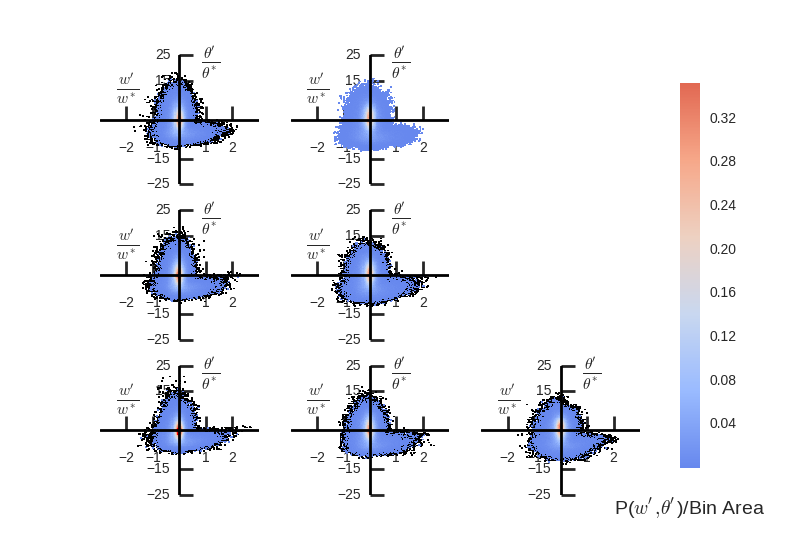
\includegraphics[scale=.76]{figures/scaled_fluxquadhist1}                 
\caption[Two-dimensional Distributions of $\frac{w^{'}}{w_{*}}$ and $\frac{\theta^{'}}{\theta_{*}}$ for all Runs]{Two-dimensional distributions of $\frac{w^{'}}{w_{*}}$ and $\frac{\theta^{'}}{\theta_{*}}$ at $h$ for $(\overline{w^{'}\theta^{'}})_{s} = 150 \ - \ 60$Wm$^{-2}$ (top - bottom) and $\gamma = 10 \ - \  2.5$Kkm$^{-1}$ (left - right) at 5 hours. There are 100 bins for each variable with bin widths varying around 0.04 and 0.27 for $w^{'}$ and $\theta^{'}$ respectively. Thick tick marks show the narrowing of the $\frac{w^{'}}{w_{*}}$ distribution where $\frac{\theta^{'}}{\theta_{*}}$ is positive, as well as the positive shift in $\frac{\theta^{'}}{\theta_{*}}$, as $\gamma$ increases.}
\label{fig:scaled_fluxquadhs}
\end{figure}

Although the quadrant of overall largest magnitude is that of upward moving cool air ($w^{'+}\theta^{'-}$), in the EZ the net heat flux is downward moving warm ($w^{'-}\theta^{'+}$) air as the other three quadrants approximately cancel.  This is in line with the findings of \cite{SullMoengStev}.  The average downward moving warm quadrant ($\overline{w^{'-}\theta^{'+}}$) at $h$ represents the pockets of trapped or engulfed warm air that become mixed into the growing CBL.  So its magnitude can be taken as a measure of entrainment.  This increases in magnitude, with time as well as with increasing $(\overline{w^{'}\theta^{'}})_{s}$.  Partitioning $(\overline{w^{'-}\theta^{'+}})_{h}$ into its velocity and temperature components reveals complexity.  The velocity component $\overline{w^{'-}}_{h}$  where $ \overline{\theta^{'}}_{h}>0$, is effectively scaled by $w_{*}$.  The curves representing $\overline{\theta^{'+}}_{h}$ where $\overline{w^{'}}_{h}<0$ vs time do not seem to collapse when scaled by $\theta_{*}$.  Figure \ref{fig:downwarm_theta} (a) shows this component is scaled effectively by the potential temperature scale introduced in Section \ref{subsubsec:tempscales}, $\delta h \gamma$.  Thus, $\gamma$ influences entrained warm air at $h$ are more significantly than $(\overline{w^{'}\theta^{'}})_{s}$.\\ 
\\   

\begin{figure}[htbp]
\begin{minipage}[b]{0.5\linewidth}
         \subfloat[]{\label{main:a}
                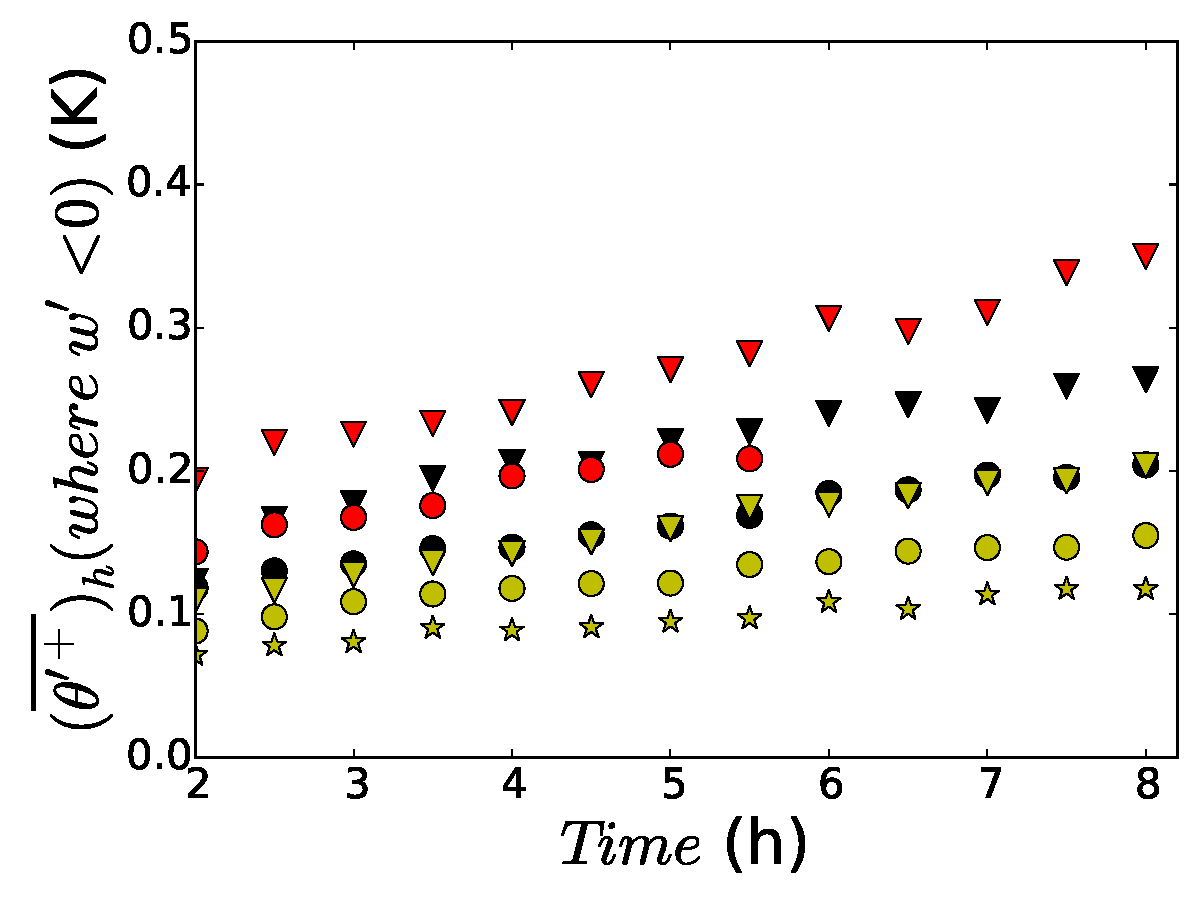
\includegraphics[scale=.3]{figures/downwarm_theta.pdf}}\\
                     
\end{minipage}             
\quad
\begin{minipage}[b]{0.5\linewidth}
         \subfloat[]{\label{main:b}          
               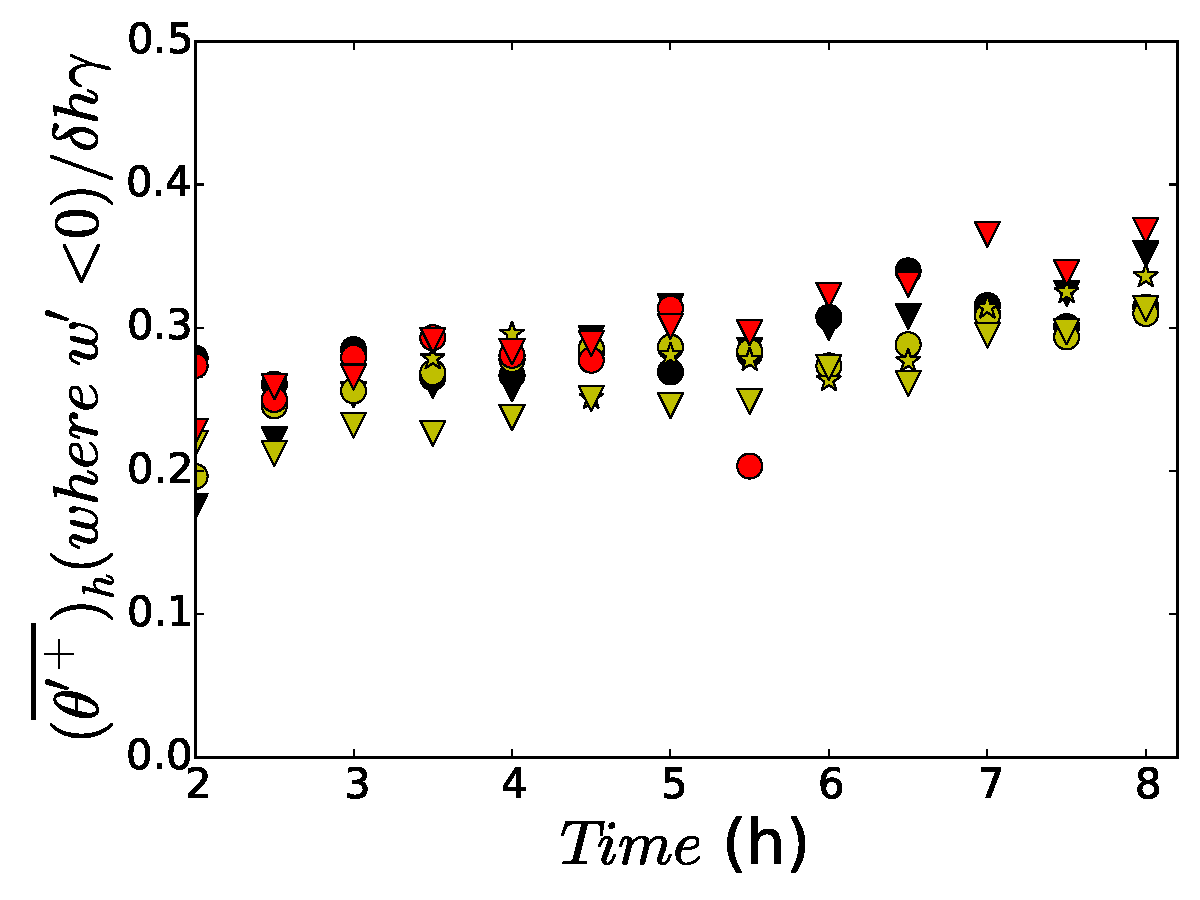
\includegraphics[scale=.3]{figures/scaled_downwarm_theta1.pdf}}\\      
       
        \end{minipage}
        \caption[Downward moving positive potential temperature fluctuations at $h$]{(a) shows $\overline{\theta^{\prime+}}_{h}$ at points where $w^{\prime}<0$ and (b) $\overline{\theta^{\prime+}}_{h}$ where $w^{\prime}<0$ scaled by $\delta h \gamma$.  Legend key:{\color{red} \ding{116}} 150/10 \hspace{3mm}{\color{red} \ding{108}} 150/5 \hspace{2mm} {\color{black} \ding{116}} 100/10 \hspace{2mm} {\color{black} \ding{108}} 100/5 \hspace{2mm} {\color{offyellow} \ding{116}} 60/10 \hspace{2mm} {\color{offyellow} \ding{108}} 60/5 \hspace{2mm} {\color{offyellow} \ding{72}} 60/2.5}
        \label{fig:downwarm_theta}
\end{figure}
\clearpage

A similar scale to $\delta h \gamma$ was introduced by \cite{GarciaMellado} to further their line of reasoning that the buoyancy in the upper EZ is determined by $\gamma$. A broad qualitative explanation is as follows: at $h$ much of the air is at the background (or initial) potential temperature $\overline{\theta}_{0}(h)$.  Some air at potential temperature $\theta = \overline{\theta}_{0}(h_{1})$ is brought down from the upper EZ limit ($h_{1}$) resulting in positive potential temperature fluctuations ($\theta^{'+}$) at $h$.\\

\subsection{EZ boundaries}

\subsubsection{Height definitions based on scaled $\overline{w^{'}\theta^{'}}$}
Neither \cite{FedConzMir04} nor \cite{GarciaMellado} define the EZ based on the $\frac{\partial \overline{\theta}}{\partial z}$ profile.  So to enable direct comparison, heights were based on the scaled heat flux ($\overline{w^{'}\theta^{'}}$) profile as in Figure \ref{fig:hdefs}. The scaled EZ depth ($\frac{z_{f0}-z_{f1}}{z_{f}}$), thus defined, remains more less constant with respect to time and shows little or no $Ri$ dependence.  This is supported by the similarity in time and across runs of the vertical heat flux profiles when scaled by $(\overline{w^{'}\theta^{'}})_{s}$.  In this definition framework \cite{FedConzMir04} showed decreasing scaled EZ with increasing $Ri$ and concluded an exponent $b = -\frac{1}{2}$.  They attributed the decrease in the overall scaled depth to a slight decrease in the scaled upper boundary over time.  However based on their plot the decrease seems more than slight, varying from about 0.5 to 0.2.  \cite{BrooksFowler2} found no clear $Ri$ dependence of the scaled EZ depth defined based on the $\overline{w^{'}\theta^{'}}$ profile.  But their definition hinged solely upon the lower part ($z_{f1} - z_{f}$) which according to \cite{FedConzMir04} does not vary in time.\\

The most obvious possible cause for disagreement with the results of \cite{FedConzMir04} described above is the difference in grid size shown in Table \ref{table:gridcomp}.  Inspection of their $\overline{w^{'}\theta^{'}}$ profiles confirms a relatively deeper scaled region of negative flux as compared with those seen here (~.4 vs ~.25). Their surface heat flux $\overline{w^{'}\theta^{'}}_{s}$ was twice the highest used here, but their range of $Ri$ is comparable to that of this study.  The latter point although not directly relevant here, serves as confirmation that $\gamma$ is the more influential parameter.\\

  
\begin{table}[htbp]
\label{table:elandri}
\caption[EZ Definitions used in comparable Studies]{EZ Definitions used in comparable Studies.  See Figure \ref{fig:hdefs}}

\begin{tabular}{ p{3.9cm} p{2.cm} p{1.cm} p{3cm}}
   

Publication & EZ Depth & CBL height & $\theta$ Jump\\ \hline
\cite{FedConzMir04} & $z_{f1} - z_{f0}$ & $z_{f}$ &  $\overline{\theta}(z_{f1})-\overline{\theta}(z_{f0})$\\ %[.3cm] %\hline
\cite{BrooksFowler2} & $2 \times (z_{f} - z_{f0})$ & $z_{f}$ & average of local values\\ \hline

\end{tabular}
    
\end{table}


\subsubsection{Heights based on scaled $\overline{\theta}$ gradient profile}

Initially, CBL height and EZ boundaries are defined based on the (unscaled) $\frac{\partial \overline{\theta}}{\partial z}$ profile.  As \cite{BrooksFowler2} pointed out, when using an average vertical tracer profile there is no universal criterion for a significant gradient.  So a threshold value for the lower EZ boundary ($h_{0}$) was chosen here, such that it was positive, small (i.e. an order of magnitude less than $\gamma$) and the same for all runs.  For the sake of rigor, plots of Eq. \ref{eq:dhvsri}
are produced based on two additional threshold values yielding analogous results.  In all three cases curves group according to $\gamma$ as shown in Fig. \ref{fig:scaleddeltahinvri} (c).\\

The importance of $\gamma$ is revealed again as the curves representing Equation \ref{eq:dhvsri} in Fig. \ref{fig:scaleddeltahinvri} (d) become similar when heights are based on the scaled profile, $\frac{\frac{\partial \overline{\theta}}{\partial z}}{\gamma}$ shown in Fig. \ref{fig:scaleddeltahinvri}. Closer inspection shows that this change primarily occurs at the lower EZ boundary ($h_{0}$) when $\frac{\partial \overline{\theta}}{\partial z}$ is scaled by $\gamma$. So the upper lapse rate influences both the vertical temperature gradient at the lower EZ boundary and the downward moving warm air at the CBL top.\\

\begin{figure}[htbp]
\begin{minipage}[b]{0.5\linewidth}
         
        \subfloat[]{\label{main:a}
                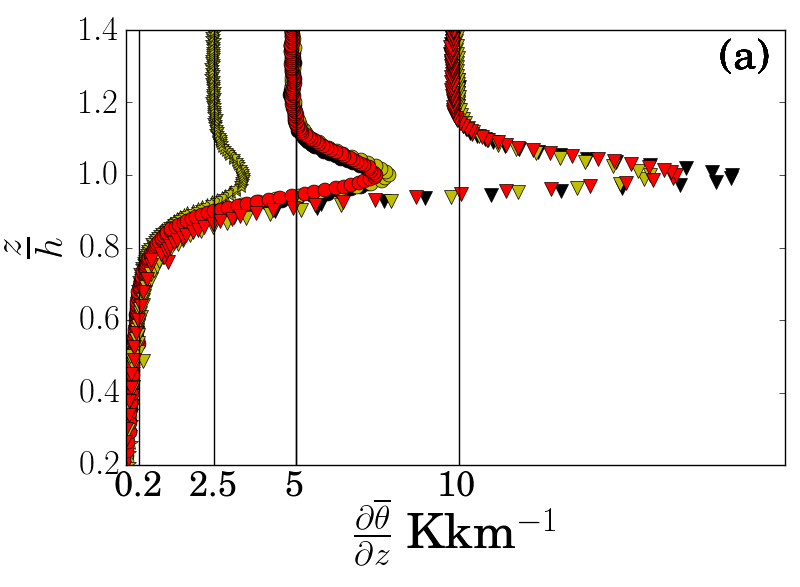
\includegraphics[scale=.3]{figures/theta_grad_profs}}\\
        \subfloat[]{\label{main:c}
                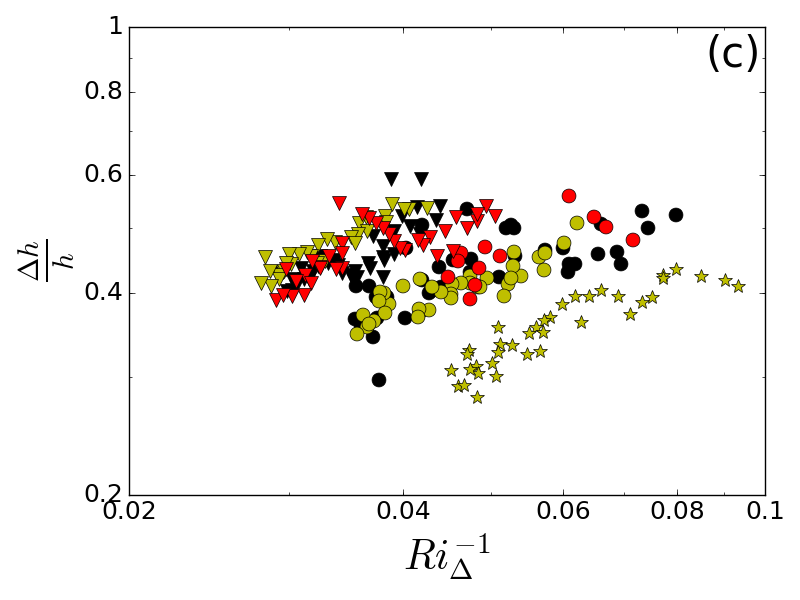
\includegraphics[scale=.3]{figures/scaleddeltahinvri}}\\
                     
\end{minipage}             
\quad
\begin{minipage}[b]{0.5\linewidth}
        \subfloat[]{\label{main:b}          
         
                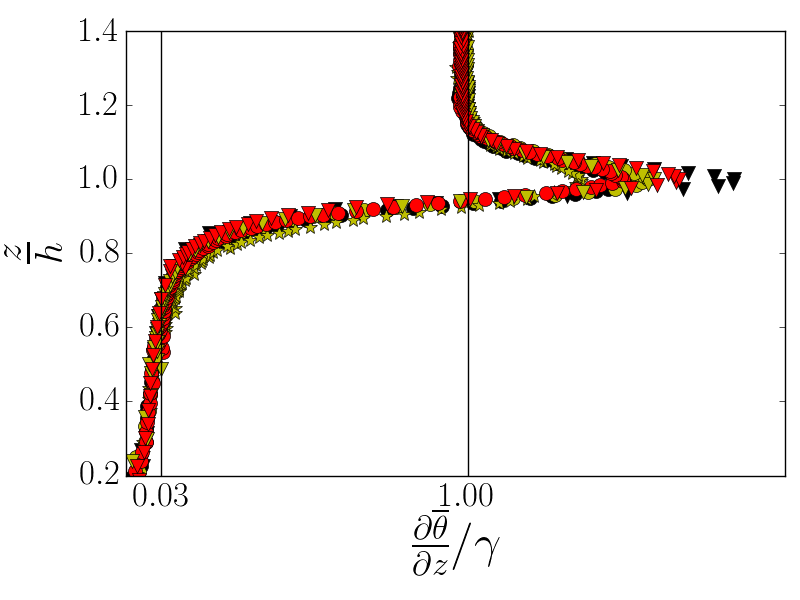
\includegraphics[scale=.3]{figures/scaled_theta_grad_profs}}\\      
        \subfloat[]{\label{main:d}          
          
                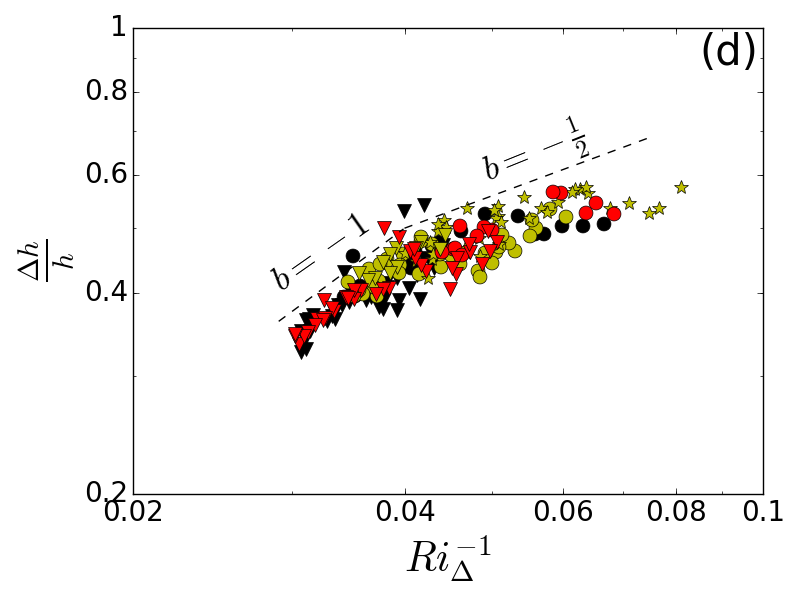
\includegraphics[scale=.3]{figures/loglog_scaleddeltahinvri_4}}\\      
       
        \end{minipage}
        \caption{The average (unscaled) vertical potential temperature gradient profiles for each run are plotted in (a) for comparison with the scaled versions ($\frac{\frac{\partial \overline{\theta}}{\partial z}}{\gamma}$) in (b).  The corresponding plots of $\frac{\Delta h}{h} \propto Ri_{\Delta} ^{b}$ are plotted in loglog coordinates in (c) and (d) to show how curves separate according to $\gamma$ when heights are based on the unscaled profile, and collapse when based on the scaled version.  Legend key:{\color{red} \ding{116}} 150/10 \hspace{3mm}{\color{red} \ding{108}} 150/5 \hspace{2mm} {\color{black} \ding{116}} 100/10 \hspace{2mm} {\color{black} \ding{108}} 100/5 \hspace{2mm} {\color{offyellow} \ding{116}} 60/10 \hspace{2mm} {\color{offyellow} \ding{108}} 60/5 \hspace{2mm} {\color{offyellow} \ding{72}} 60/2.5.}
        \label{fig:scaleddeltahinvri}
\end{figure}


These results support a varying exponent $b$ in Equation \ref{eq:dhvsri} which is lower in magnitude ($-\frac{1}{2}$) at lower $Ri$ and approaches $-1$ at higher $Ri$.  This is in line with theory and the results of comparable studies so the EZ boundary definitions based on the $\frac{\frac{\partial \overline{\theta}}{\partial z}}{\gamma}$ profile are valid.  Overall there is a clear narrowing of the scaled EZ depth with increasing $Ri$ (decreasing $Ri^{-1}$) as supported by the local height distributions in Section \ref{subsubsec:loccblh}.  Although based on different height definitions, \cite{FedConzMir04} concluded an exponent $b = -\frac{1}{2}$ and \cite{BrooksFowler2}'s plots show curves with an apparent exponent less in magnitude than $-1$.  Their curves representing each run fanned out.  Here, before scaling by $\gamma$, the curves representing Eq. \ref{eq:dhvsri} using height definitions based on $\frac{\partial \overline{\theta}}{\partial z}$ separate out, but in the reverse order.  Increased stability, ie higher $Ri$, causes larger scaled EZ depths.  Whereas \cite{BrooksFowler2}'s runs with initially lower $Ri$ had larger scaled EZ depths than those with higher, even where $Ri$ values overlap. Nonetheless, that there appears a family of separate but similar curves rather than a single curve hints at an underlying scaling parameter.\\     

\cite{GarciaMellado} suggested that the buoyancy in the lower portion of the EZ, i.e. from a point just below $h$ down, is more strongly influenced by the vigorous turbulence of the ML than by $\gamma$.  So mixing reduces the difference between, the potential temperature at the top of the ML, and that at or just below $h$.  However, that the magnitude of the average vertical potential temperature gradient ($\frac{\partial \overline{\theta}}{\partial z}$) in the upper ML increases with increasing $\gamma$, indicates that the influence of this parameter extends further down.\\

None of the other comparable studies clearly address the change in exponent with increased $Ri$ observed in Fig. \ref{fig:scaleddeltahinvri} (d).  It is possible that this represents a change in entrainment mechanism. \cite{SullMoengStev} observed enfolding and engulfment at lower $Ri$.  Whereas at higher $Ri$ when motion is more restricted, entrainment seemed to occur via trapping of thinner wisps at the edge of an upward moving thermal.  \cite{Turner86} also distinguishes between entrainment by convective overturning and recoil. \cite{GarciaMellado} refer to a change in entrainment rate due to the effects of increased stability on the upper EZ sub-layer.  In this study, the narrowing of the EZ depends predominantly on the magnitude of the average vertical potential temperature gradient $\frac{\partial \overline{\theta}}{\partial z}$ in the lower EZ and upper ML.  However, the scaled magnitude of upper limit does appear to decrease slightly in time.  This could correspond to the slowly decreasing upper sub layer of the EZ mentioned in both \cite{GarciaMellado} and \cite{FedConzMir04}.\\

\subsection{Entrainment rate}

$Ri$ magnitude determined in this and the comparable studies is primarily influenced by the magnitude of the $\theta$ jump.  Here, it is defined in two ways as \cite{FedConzMir04} did.  The heights and $\theta$ jump are based on the scaled $\overline{w^{'}\theta^{'}}$ profile aswell as the scaled $\overline{\theta}$ gradient profile (Figure \ref{fig:hdefs} and Table \ref{tab:reldefs}).  This multitude of definitions enables comparison and observation of how the $\theta$ jump definition effects Equation \ref{eq:ervsri}.

\subsubsection{Height definitions based on scaled $\overline{w^{'}\theta^{'}}$}
In Fig. \ref{fig:weinvri} the axes are in log-log coordinates and all heights are based on the scaled $\overline{w^{'}\theta^{'}}$ profile. The relationship of scaled entrainment rate to $Ri_{\Delta}$ in (a) could fit either value of $a$ or a value in between.  The larger jump, i.e. that taken across the EZ ($\Delta \theta$), yields a larger value of $a$ as \cite{FedConzMir04} concluded.  \cite{GarciaMellado} interpreted both curves as asymptotic to straight lines ($a=-1$) as the upper EZ sub-layer narrows.  These straight lines are plotted in Fig. \ref{fig:weinvri} (a) and (b) indicating that their DNS results have been reproduced here.   Plot (a) for $\delta \theta$ in Figure \ref{fig:weinvri} could also represent a curve with exponent less in magnitude than $-1$ initially.  Plot (b) for $\Delta \theta$ could represent a curve with increasing exponent exceeding magnitude $-1$ at higher $Ri$.\\

\begin{figure}[htbp]
\begin{minipage}[b]{0.5\linewidth}
        
        \subfloat[]{\label{main:a}
                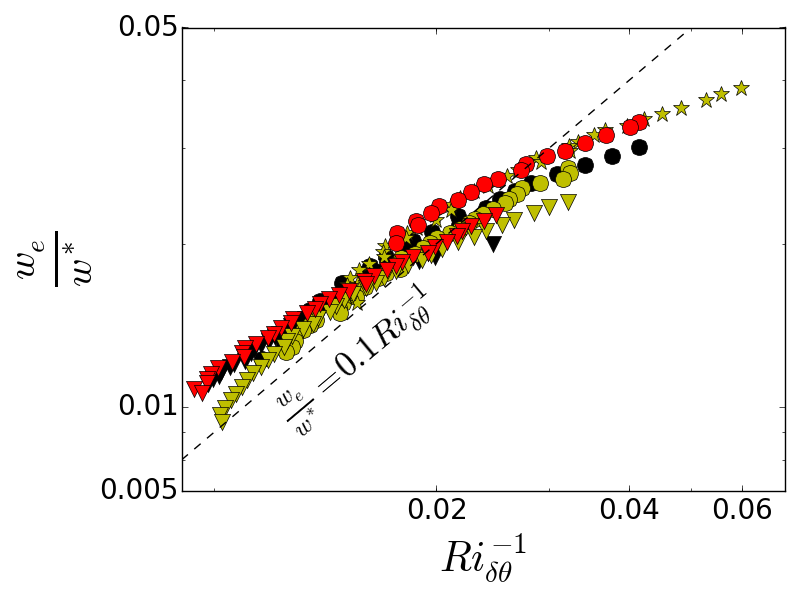
\includegraphics[scale=.3]{figures/scaledweinvri_delta_f_GM.png}}\\
        \subfloat[]{\label{main:b}
                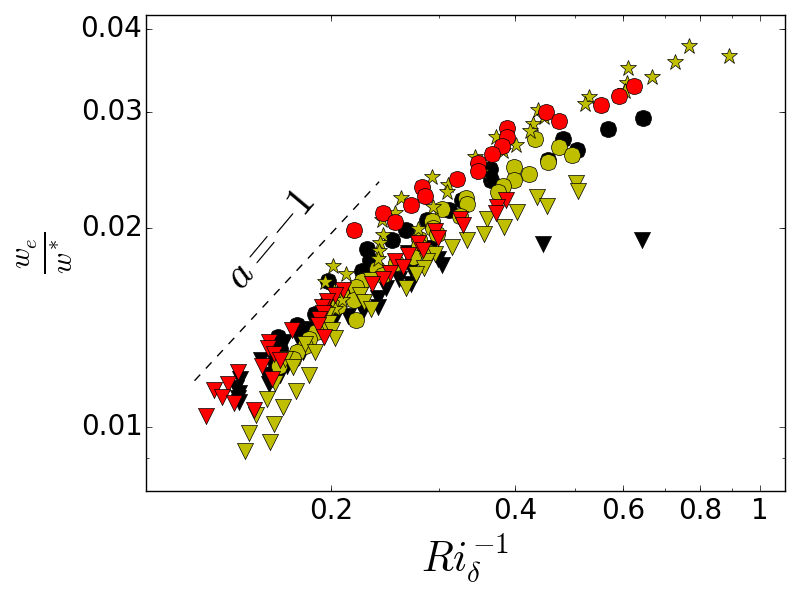
\includegraphics[scale=.3]{figures/scaledweinvri_delta.png}}\\
                     
\end{minipage}             
\quad
\begin{minipage}[b]{0.5\linewidth}
        \subfloat[]{\label{main:c}          
          
                %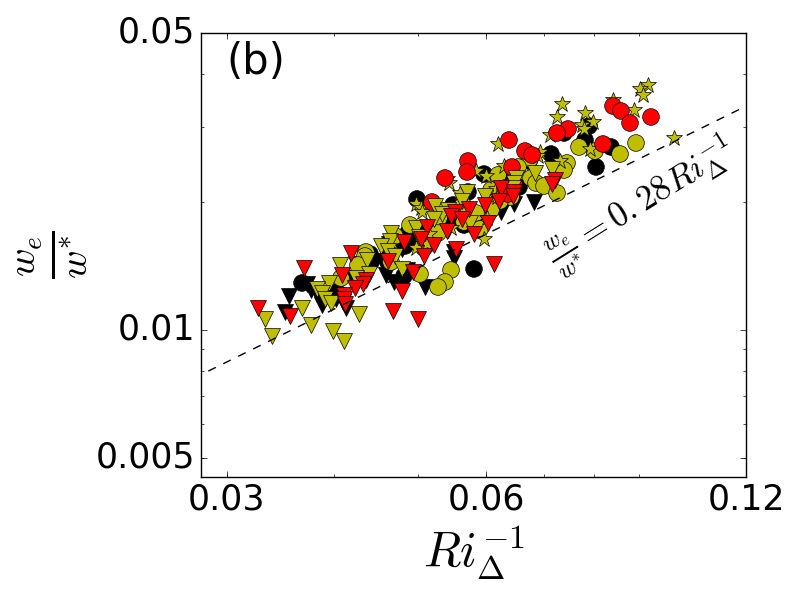
\includegraphics[scale=.3]{figures/scaledweinvri_Delta_f_GM}
}\\      
        \subfloat[]{\label{main:d}          
          
                %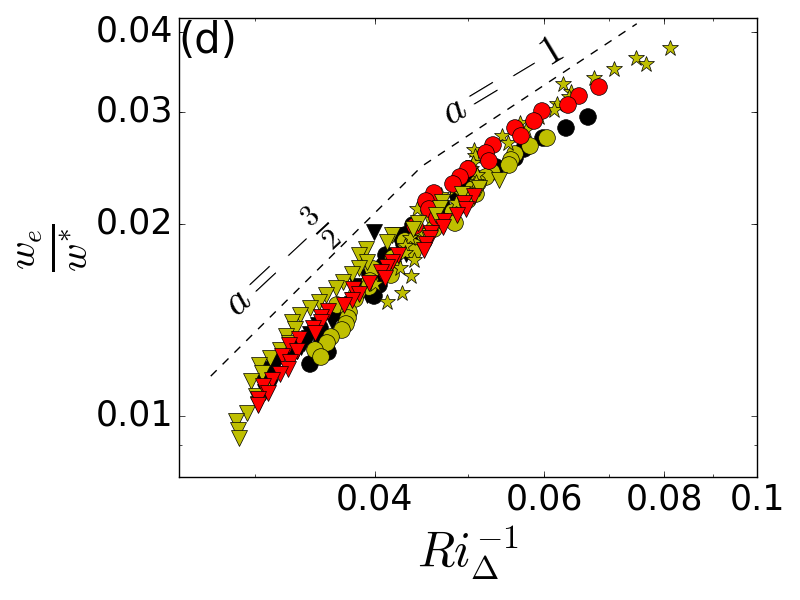
\includegraphics[scale=.3]{figures/scaledweinvri_Delta}
}\\      
       
        \end{minipage}
        \caption{Plots of $\frac{w_{e}}{w_{*}} \propto Ri^{a}$ using height definitions based on the scaled vertical heat flux profile with straight lines predicted by \cite{GarciaMellado} are in (a) and (b).  (c) and (d) show this relationship when heights are based on the scaled average potential temperature gradient profile. In both sets of plots $\Delta$ represents the temperature jump accross the EZ whereas $\delta$ represents that taken at the CBL top. Legend key:{\color{red} \ding{116}} 150/10 \hspace{3mm}{\color{red} \ding{108}} 150/5 \hspace{2mm} {\color{black} \ding{116}} 100/10 \hspace{2mm} {\color{black} \ding{108}} 100/5 \hspace{2mm} {\color{offyellow} \ding{116}} 60/10 \hspace{2mm} {\color{offyellow} \ding{108}} 60/5 \hspace{2mm} {\color{offyellow} \ding{72}} 60/2.5}
        \label{fig:weinvri}
\end{figure}


\subsubsection{Height definitions based on $\frac{\frac{\partial \overline{\theta}}{\partial z}}{\gamma}$ profile}
In Figure \ref{fig:weinvri} (c) and (d) all heights are based on the $\frac{\frac{\partial \overline{\theta}}{\partial z}}{\gamma}$ profile.  Again, there is a difference in exponent when $\Delta \theta$ is used as compared to when $\delta \theta$ is used.  In Fig. \ref{fig:weinvri} (c) $a=-\frac{3}{2}$ fits at higher $Ri$ (lower $Ri^{-1}$) and $a=-1$ seems to fit at lower $Ri$.  Combined with the apparent change in $b$ for Equation \ref{eq:dhvsri}, this is interpreted as an indication of entrainment regime change with increasing $Ri$.\\ 


\section{Conclusions}
\subsection{The turbulence causing entrainment in the EZ is adequately resolved using LES at the resolution used in this study.}

According to FFT energy density spectra the modeled domain has a realistic inertial subrange.  The dominant energy containing structures in the EZ are smaller, and decay to the smallest resolved turbulent structures is steeper. This is consistent with the assertion of \cite{GarciaMellado} that the EZ is separated into two sub-layers in terms of turbulence scales.  Several individual, coherent, thermals are seen at any given time, indicating that realistic turbulence is being simulated.  The relationship of scaled entrainment rate to $Ri$ shown in the DNS study of \cite{GarciaMellado} appears to be reproduced here, even when the $\theta$ jump is defined across the EZ.  This indicates that the dominant processes causing entrainment are represented as effectively in this study as in their DNS study.

\subsection{The gradient method for determining local CBL height, based on the potential temperature profile, is conceptually and practically flawed.  A regression or curve fitting method is better.}

Local $\theta$ profiles vary depending on location.  The top of an active thermal impinging on the free atmosphere (FA) as in Fig. \ref{fig:rssfitshigh} is characterized by a steep gradient comparable to the zero-order model representation.  At other locations, for example where a thermal has overturned or recoiled and some entrainment has been initiated as in Fig. \ref{fig:rssfitshigh}, there is a region over which the $\theta$ profile transitions to the upper lapse rate ($\gamma$). That is, there is a local entrainment zone (EZ).  At such locations, there are gradients well into the FA that exceed any within the EZ, as well as an absence of a well-defined local CBL height.  This presents both a practical and conceptual challenge to the gradient method.  Based on hundreds of individual local $\theta$ profiles, determination of the ML height using piecewise linear regression makes more sense visually and is more reliable. 

\subsection{The scaled average vertical potential temperature profile is a valid framework for defining CBL height and EZ boundaries}

The $\overline{\theta}$ profile characterizes the dry, idealized CBL and links bulk models to soundings via an LES.  Both the EZ depth and CBL height based on the average $\frac{\frac{\partial \overline{\theta}}{\partial z}}{\gamma}$ profile showed dependence on $Ri$ as seen in other studies and justified theoretically.  So this is a valid way of defining the CBL and its EZ.  

\subsection{Once average vertical surface heat flux is accounted for by $h$, $\gamma$ dominates CBL entrainment, so should be included in any set of scales representing this region.}

The magnitude and variance of local ML height, increase with increasing $\overline{w^{'}\theta^{'}}_{s}$, and decrease with increasing $\gamma$.  The same can be said for the vertical velocity fluctuations ($w^{'}$) in the EZ.  However, increased $\gamma$ results in an increase in the positive potential temperature fluctuations ($\theta^{'+}$) at $h$. The magnitude of ($\theta^{'+}$) at points where $w^{'}$ is negative represents downward moving entrained air and depends on $\gamma$.  Below $h$, in the lower EZ, the average vertical potential temperature gradient ($\frac{\partial \overline{\theta}}{\partial z}$) also depends on $\gamma$. So, the growth of the idealized dry CBL is driven by $(\overline{w^{'}\theta^{'}})_{s}$ and suppressed by stability ($\gamma$). But CBL warming is due, in part, to the entrainment of air from aloft the potential temperature of which in turn depends on $\gamma$.\\

Evidence for the influence of $\gamma$ is seen throughout this study.  Distributions of scaled local ML heights approach similarity, when $\gamma$ is constant but $(\overline{w^{'}\theta^{'}})_{s}$ is varied.  Curves representing Equation \ref{eq:dhvsri} group according to $\gamma$ when based on the $\frac{\partial \overline{\theta}}{\partial z}$ profile, but collapse once based on $\frac{\frac{\partial \overline{\theta}}{\partial z}}{\gamma}$.  The convective time scale $\tau = \frac{w_{*}}{h}$ and $Ri$ group according to $\gamma$ lending support to \cite{FedConzMir04}'s use of the Brunt-V{\"a}is{\"a}l{\"a} time scale.  It seems that once the effect of the surface heat flux ($\overline{w^{'}\theta^{'}}_{s}$) is accounted for through $h$, $\gamma$ emerges as the dominant parameter in dry, idealized CBL entrainment.\\
 
\subsection{$Ri$ dependence of the scaled EZ depth and entrainment rate changes as $Ri$ increases.}

\cite{Turner86} outlined and theoretically justified two distinct convective boundary layer entrainment regimes wherein the scaled entrainment rates have different $Ri$ dependence. The LES flow visualizations of \cite{SullMoengStev} showed large scale engulfment at lower $Ri$.  At higher $Ri$, trapping of smaller volumes of stable air between and at the edges of impinging thermals appeared to be the dominant mechanism. The CBL entrainment zone measurements analyzed in \cite{Traum11} further support the concept of varying entrainment mechanism depending on the strength of the upper lapse rate $\gamma$.  Finally, both \cite{FedConzMir04} and \cite{GarciaMellado} discuss the varying dependence of the scaled entrainment rate on $Ri$ as the effects of upper stability become more important.  On these grounds the change in exponent in the plots of equations \ref{eq:dhvsri} and \ref{eq:ervsri} in Figures \ref{fig:deltahinvri} and \ref{fig:weinvri} can be attributed to a change in entrainment regime as $Ri$ increases.   



\begin{acknowledgements}
NSERC CREATE-AAP and NSERC Discovery grants to Douw Steyn and Phil Austin (funding), Compute Canada (computational resources), Python, Matplotlib, Scipi, Cython, Constantine Evans (scikits-bootstrap) 
\end{acknowledgements}


% BibTeX users please use one of
\bibliographystyle{spbasic}      % basic style, author-year citations
%\bibliographystyle{spmpsci}      % mathematics and physical sciences
%\bibliographystyle{spphys}       % APS-like style for physics
\bibliography{nchap_sub}   % name your BibTeX data base




\end{document}
% end of file template.tex

